\documentclass[11pt]{article}
\def\activityid{ADULT GUIDE}
% Shared style and exact pattern-block geometry. Compile with pdfLaTeX.
\usepackage[letterpaper,margin=0.65in,top=0.60in,bottom=0.65in]{geometry}
\usepackage[T1]{fontenc}
\usepackage[default]{sourcesanspro}
\usepackage{microtype,tikz,array,tabularx,fancyhdr}
\usepackage[hidelinks]{hyperref}
\usetikzlibrary{calc}
\setlength{\parindent}{0pt}
\setlength{\parskip}{7pt}
\setlength{\headheight}{0pt}
\setlength{\footskip}{26pt}
\setlength{\emergencystretch}{2em}
\pagestyle{fancy}\fancyhf{}
\renewcommand{\headrulewidth}{0pt}
\renewcommand{\footrulewidth}{0.4pt}
\fancyfoot[L]{\scriptsize Bellingham Math Circle\enspace /\enspace Week 1\enspace /\enspace \activityid}
\fancyfoot[R]{\scriptsize \thepage}
\definecolor{ink}{gray}{0.12}
\definecolor{soft}{gray}{0.95}
\color{ink}
\newlength{\blockside}
\setlength{\blockside}{1in} % Change here if your blocks have another edge length.
\def\hh{0.8660254037844386}
\tikzset{outline/.style={draw=ink,line width=1.1pt,line join=round},
  tile/.style={draw=ink,line width=0.65pt,line join=round,fill=white},
  tilelabel/.style={font=\bfseries\small,inner sep=1pt}}
\newcommand{\HexPath}{(-1,0)--(-.5,-\hh)--(.5,-\hh)--(1,0)--(.5,\hh)--(-.5,\hh)--cycle}
\newcommand{\PennantPath}{(-1,0)--(-.5,-\hh)--(.5,-\hh)--(1,0)--(.5,\hh)--(0,2*\hh)--(-.5,\hh)--cycle}
\newcommand{\DoublePath}{(-1,0)--(-.5,-\hh)--(.5,-\hh)--(1,0)--(.5,\hh)--(1,2*\hh)--(.5,3*\hh)--(-.5,3*\hh)--(-1,2*\hh)--(-.5,\hh)--cycle}
\newcommand{\BluePath}{(-.75,-.5*\hh)--(.25,-.5*\hh)--(.75,.5*\hh)--(-.25,.5*\hh)--cycle}
\newcommand{\RedPath}{(-1,-.5*\hh)--(1,-.5*\hh)--(.5,.5*\hh)--(-.5,.5*\hh)--cycle}
\newcommand{\DrawOutline}[1]{\begin{tikzpicture}[x=\blockside,y=\blockside]\draw[outline] #1;\end{tikzpicture}}
\newcommand{\PageTitle}[2]{
  {\fontsize{10}{12}\selectfont\bfseries WEEK 1\quad PATTERN BLOCKS\hfill #1\par}
  \vspace{3pt}{\fontsize{27}{30}\selectfont\bfseries #2\par}\vspace{2pt}}
\newcommand{\NameLine}{{\small Name: \rule{2.65in}{.4pt}\hfill Date: \rule{1.35in}{.4pt}\par}\vspace{4pt}}
\newcommand{\Task}[2]{\par\vspace{3pt}{\large\bfseries #1}\par #2\par}
\newcommand{\RuleBox}[1]{\par\begingroup\setlength{\fboxsep}{8pt}\colorbox{soft}{\parbox{\dimexpr\linewidth-16pt\relax}{#1}}\endgroup\par}
\newcommand{\WriteBox}[2]{\par\textbf{#1}\par\vspace{2pt}\begin{tikzpicture}\draw[draw=black!40,line width=.5pt] (0,0) rectangle (\dimexpr\linewidth-.5pt\relax,#2);\end{tikzpicture}\par}
\newcommand{\Pair}[1]{
  \par\vspace{3pt}\noindent
  \begin{minipage}[t]{.485\linewidth}\centering\textbf{Copy A}\par\vspace{8pt}\DrawOutline{#1}\end{minipage}\hfill
  \begin{minipage}[t]{.485\linewidth}\centering\textbf{Copy B}\par\vspace{8pt}\DrawOutline{#1}\end{minipage}\par\vspace{4pt}}
\newcommand{\ColorLists}{\begin{tabularx}{\linewidth}{@{}X X@{}}
  Colors in A: \hrulefill & Colors in B: \hrulefill
  \end{tabularx}\par}
\newcommand{\PieceCounts}{\begin{tabularx}{\linewidth}{@{}X X X@{}}
  Pieces in A: \hrulefill & Pieces in B: \hrulefill & Total: \hrulefill
  \end{tabularx}\par}
\newcommand{\ScaleCheck}{\vfill\par\begingroup\fontsize{9}{11}\selectfont
  \begin{minipage}[c]{1.2in}\centering
  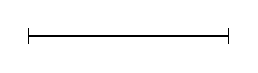
\begin{tikzpicture}[x=\blockside,y=1in]\draw[line width=.65pt] (0,0)--(1,0);\draw (0,-.04)--(0,.04) (1,-.04)--(1,.04);\end{tikzpicture}\par
  One block edge
  \end{minipage}\hfill
  \begin{minipage}[c]{\dimexpr\linewidth-1.35in\relax}
  Adult: print at \textbf{100\% / Actual Size}, single-sided. This line is 1 inch (25.4 mm) in the default file. Match a green triangle's edge to it before using the mats.
  \end{minipage}\par\endgroup}
\newcommand{\StudentFooter}{\vfill{\small Build first. You may explain by pointing, talking, or drawing.}\par}
\newcommand{\Allowed}{{\small Use only green triangles, blue rhombi, red trapezoids, and yellow hexagons.\par}}
\newcommand{\CoverRule}{Cover each outline exactly: no gaps, overlaps, or pieces outside.}
\newcommand{\ColorRule}{Keep both copies built. A color used in A cannot be used in B.}
% Small labeled diagrams for adult solutions only; these are not actual-size mats.
\newcommand{\Tile}[3]{\path[tile] #1;\node[tilelabel] at #2 {#3};}
\newcommand{\PoneYG}{
 \Tile{\HexPath}{(0,0)}{Y}
 \Tile{(-.5,\hh)--(.5,\hh)--(0,2*\hh)--cycle}{(0,1.3333*\hh)}{G}}
\newcommand{\PoneRBB}{
 \Tile{(0,0)--(.5,\hh)--(0,2*\hh)--(-.5,\hh)--cycle}{(0,\hh)}{B}
 \Tile{(0,0)--(.5,-\hh)--(1,0)--(.5,\hh)--cycle}{(.5,0)}{B}
 \Tile{(-.5,\hh)--(-1,0)--(-.5,-\hh)--(.5,-\hh)--cycle}{(-.4,-.3*\hh)}{R}}
\newcommand{\HexReds}{
 \Tile{(-1,0)--(1,0)--(.5,\hh)--(-.5,\hh)--cycle}{(0,.43*\hh)}{R}
 \Tile{(-1,0)--(-.5,-\hh)--(.5,-\hh)--(1,0)--cycle}{(0,-.43*\hh)}{R}}
\newcommand{\HexBlues}{
 \Tile{(0,0)--(1,0)--(.5,\hh)--(-.5,\hh)--cycle}{(.25,.5*\hh)}{B}
 \Tile{(0,0)--(-.5,\hh)--(-1,0)--(-.5,-\hh)--cycle}{(-.5,0)}{B}
 \Tile{(0,0)--(-.5,-\hh)--(.5,-\hh)--(1,0)--cycle}{(.25,-.5*\hh)}{B}}
\newcommand{\DoubleTiles}[1]{#1\begin{scope}[shift={(0,2*\hh)}]#1\end{scope}}
\newcommand{\SolutionPic}[1]{\begin{tikzpicture}[x=.54in,y=.54in]#1\end{tikzpicture}}

\hypersetup{pdftitle={Week 1: Pattern blocks - facilitator guide and solutions},pdfauthor={Bellingham Math Circle}}
\newcommand{\Subhead}[1]{\par\vspace{4pt}{\large\bfseries #1}\par}
\begin{document}
\PageTitle{FACILITATOR}{Week 1: block trades}
\textbf{Mathematical idea:} The same boundary can have different decompositions. A color restriction links two constructions; area helps explain a minimum.
\RuleBox{\textbf{Use these as building mats.} Allow free play before handing out the first task. Give one page at a time; the later pages are invitations, not a completion requirement. Children may point, speak, or build instead of writing.}
\Subhead{Print and prepare}
Print student packets \textbf{single-sided on US Letter at 100\% / Actual Size}. Turn off ``Fit'' or ``Shrink.'' Each mat assumes a \textbf{1-inch (25.4 mm) block edge}. Compare the check line with an actual green triangle before the session. If your blocks differ, trace around the actual blocks on blank paper, or change \texttt{\textbackslash blockside} in \texttt{common.tex} and rebuild; recheck page fit.

The K--1 packet has 2 pages; grades 2--3 and 4--5 have 3 each. For the current roster, print 3 K--1 packets, 3 middle packets, and 1 upper packet (18 student sheets). Keep this answer guide with the adults.

Per child, aim for \textbf{2 yellow, 4 red, 6 blue, and 8 green blocks}, with spare greens. Use only the green equilateral triangle, blue 60-degree rhombus, red trapezoid, and yellow hexagon. Set squares and thin rhombi aside. Add pencils, scrap paper, and optional sleeves. No color printing is needed: outlines are black and white. If colors are difficult to distinguish, use the shape names or G/B/R/Y labels; treat the restriction as ``no block type in both copies.''
\Subhead{Choose an entry point}
\begin{tabularx}{\linewidth}{@{}p{.62in}X@{}}
\textbf{K--1} & Match edges and turn pieces; no reading, writing, or arithmetic required. Start with a single blue or red outline. Count only if useful.\\[5pt]
\textbf{2--3} & Track block types across two copies; small counts are optional. Read prompts aloud as needed. Allow shared colors first, then fix one shared type at a time.\\[5pt]
\textbf{4--5} & Add small piece counts and compare an example with a claim about every possible pair. No area formulas or multiplication tables required. Enter through the middle task if helpful.
\end{tabularx}
\Subhead{A flexible hour}
\textbf{0--10:} Free building. \textbf{10--15:} Trace or show the blue outline; remove the block and ask, ``Can you change the pieces without changing the shape?'' Check one complete trade together. \textbf{15--35:} Start each group's first page. \textbf{35--40:} Move/reset. \textbf{40--55:} Continue a good investigation or offer the next page. \textbf{55--60:} Show one discovery and tidy up.

Keep one parent mainly with K--1. The organizer launches the middle group and the fifth grader, then returns to each regularly. Give each child a set of blocks and building space. Reserve a conversation with the fifth grader about whether a smaller pair is possible.

\textbf{Play exchange shop:} A partner brings a block; the shopkeeper trades it for smaller pieces covering the same space. Check the trade, then swap roles.

\textbf{Useful questions:} What have you tried? Did the outside change? Which colors must the other copy avoid? Can changing a group of pieces help? Let children demonstrate checks before supplying a hint.
\newpage
\PageTitle{FACILITATOR}{Checked constructions}
\textbf{Diagram key:} G = green triangle; B = blue rhombus; R = red trapezoid; Y = yellow hexagon. The diagrams below are reduced size. Student mats show only the outside boundary.
\Subhead{K--1 trades / F01-K}
One blue rhombus trades for \textbf{two greens}. One red trapezoid trades for \textbf{one blue and one green}, or \textbf{three greens}. A fair trade covers exactly the same space. Place the original block over a replacement to compare. Turning an unchanged single piece does not make a new decomposition.

For the pennant, yellow + green and two reds + green give two fillings; shared colors are allowed at this level. Split the yellow hexagon into its top and bottom red trapezoids to make the second filling.
\Subhead{P1: the pennant / F01-M and F01-U}
The outline is a hexagon with a green triangle attached outside one full edge. A legal pair uses \textbf{yellow + green / red + two blues}: 2 + 3 = \textbf{5 pieces}.
\begin{center}
\begin{minipage}[b]{.32\linewidth}\centering\SolutionPic{\PoneYG}\par\textbf{Copy A: Y + G}\end{minipage}\hspace{.6in}
\begin{minipage}[b]{.32\linewidth}\centering\SolutionPic{\PoneRBB}\par\textbf{Copy B: R + B + B}\end{minipage}
\end{center}
\textbf{Hint ladder:} Keep A as yellow + green. B may use only red and blue. Join the outside triangle to the inside triangle that touches its base: together they form a blue rhombus. The remaining region takes a red and a blue, as drawn.
\Subhead{P2: double hexagon / F01-M and F01-U}
The two hexagons share one full edge. With yellow allowed, use \textbf{two yellows / four reds} (6 total). With yellow banned, use \textbf{four reds / six blues} (10 total). The same red construction works in both pairs.
\begin{center}
\begin{minipage}[b]{.30\linewidth}\centering\SolutionPic{\DoubleTiles{\Tile{\HexPath}{(0,0)}{Y}}}\par\textbf{2 yellows}\end{minipage}\hfill
\begin{minipage}[b]{.30\linewidth}\centering\SolutionPic{\DoubleTiles{\HexReds}}\par\textbf{4 reds}\end{minipage}\hfill
\begin{minipage}[b]{.30\linewidth}\centering\SolutionPic{\DoubleTiles{\HexBlues}}\par\textbf{6 blues}\end{minipage}
\end{center}
\textbf{Hint:} Fill each hexagon separately, then keep the outside and change the pieces. Check both the geometric fit and the color rule.
\newpage
\PageTitle{FACILITATOR}{Why fewer cannot work}
\Subhead{Let the units come from the blocks}
After children have tried, cover each block with green triangles. Their areas, measured in green triangles, are \textbf{G = 1, B = 2, R = 3, Y = 6}. P1 has area \textbf{7}; P2 has area \textbf{12}. Children can make the following arguments with blocks or drawings. A correct area sum alone does not prove a tiling exists; the constructions on page 2 supply that check.
\Subhead{P1: the minimum is 5 pieces across the pair}
Each copy needs at least two pieces because even the largest block covers only 6 triangle units. To cover 7 with two blocks, the only possible areas are 6 + 1: yellow + green. A four-piece pair would therefore need yellow + green in \emph{both} copies, breaking the color rule. At least 5 pieces are needed, and the illustrated pair uses 5.
\Subhead{P2: the minimum is 6 pieces across the pair}
If one copy uses yellow, it needs at least 2 pieces. The other copy cannot use yellow, so each of its pieces covers at most 3 triangle units. That copy needs at least 4 pieces. Total: at least 2 + 4 = 6.

If neither copy uses yellow, each needs at least 4 pieces, already at least 8 total. Thus no pair can beat 6; two yellows / four reds achieves 6.
\Subhead{P2 without yellow: the minimum is 10 pieces}
At most one copy may use red. If a copy uses red, its pieces cover at most 3 units each, so it needs at least 4. The other copy has only blue and green, covering at most 2 units per piece, so it needs at least 6. Total: at least 10. If neither copy uses red, each needs at least 6 pieces, giving at least 12 total. Four reds / six blues attains 10.
\Subhead{Extensions, recording, and sources}
\textbf{Keep an open question open.} A child's new outline may have an interesting construction without a proven minimum. Record ``best so far'' until there is a reason that every smaller count fails. Children may create an outline, verify two fillings, and exchange just the traced boundary.

\textbf{Prior use:} Lowell Handout 3, problem 3.4, used hexagon decompositions; Handout 4, problems 4.3--4.5, and \emph{Pattern Block Exercises}, problems 2--4 (PDF pp. 1--2), used trapezoid tilings. Give returning children the new P1/P2 constraints or minimization work. After the session, record the actual trades, P1/P2 pages, color restrictions, and arguments encountered by each child in \texttt{plans/fall-k-5-year-a-use-log.md}. Preparing these sheets does not mark them as taught.

\textbf{Activity sources:} JRMF, \emph{Changing Colors Activity Guide}, PDF pp. 3--6, supplies simultaneous copies with no shared colors and an exploration-first launch. Its \emph{Beginner Version}, PDF pp. 3--6, supplies different fillings without the color restriction. P1/P2 and the minimum-piece sequence come from this repository's \emph{Fall Year A activity guide}, Week 1, F01-K/M/U; they are local constructions, not copied JRMF task sheets.

\textbf{Format source:} \emph{Math Circle by the Bay}, preface, printed pp. ix--x (PDF pp. 10--11), describes manipulatives, extra challenges, practicing explanations, and adjusting depth across ages. Our one-page-at-a-time packets and two-adult hour are local adaptations, not a schedule prescribed by that book.
\end{document}
